\documentclass[12pt,a4paper]{article}
\usepackage[utf8]{inputenc}
\usepackage[T1]{fontenc}
\usepackage[spanish]{babel}
\usepackage{amsmath,amssymb}
\usepackage{graphicx}
\usepackage{hyperref}
\usepackage{geometry}
\geometry{margin=2.5cm}

\title{Estructura de Bandas Fotónicas Dispersivas:\\
Formulación Hermitiana con Campos Auxiliares}
\author{Codigo\_Hermitian --- Implementación Python}
\date{\today}

\begin{document}
\maketitle

\begin{abstract}
Implementación numérica del método de Raman y Fan para calcular estructuras
de bandas en cristales fotónicos con materiales dispersivos tipo Lorentz/Drude.
El problema se formula como $\omega A x = B x$ con $A$ definida positiva y
$B$ Hermitiana, resuelto mediante \texttt{scipy.sparse.linalg.eigsh} con
transformación shift-invert. Se incluyen validaciones de hermiticidad,
ortogonalidad modal y comparación perturbativa de pérdidas.
\end{abstract}

\section{Introducción}

Los metamateriales plasmónicos presentan permitividad dependiente de la
frecuencia. La dependencia $\varepsilon(\omega)$ destruye la hermiticidad
del operador de Maxwell estándar. Raman y Fan~\cite{Raman2010} introducen
campos auxiliares mecánicos acoplados a las ecuaciones de Maxwell, obteniendo
un problema de autovalores lineal Hermitiano en el caso sin pérdidas.

\section{Formulación matemática}

\subsection{Modelo de Lorentz}

\begin{equation}
  \varepsilon(\omega) = \varepsilon_\infty
  \left(1 + \frac{\omega_p^2}{\omega_0^2 - \omega^2 + i\gamma\omega}\right)
\end{equation}

\subsection{Ecuaciones acopladas}

Con convención temporal $e^{-i\omega t}$:
\begin{align}
  \partial_t H &= -\frac{1}{\mu_0}\nabla\times E, \\
  \partial_t E &= \frac{1}{\varepsilon_\infty}(\nabla\times H - V), \\
  \partial_t P &= V, \\
  \partial_t V &= \omega_p^2\varepsilon_\infty E - \omega_0^2 P - \gamma V.
\end{align}

En estado estacionario, el sistema $\omega A x = B x$ tiene
$A = \mathrm{diag}(\mu_0, \varepsilon_\infty, \omega_0^2/(\omega_p^2\varepsilon_\infty), 1/(\omega_p^2\varepsilon_\infty))$.

\subsection{Transformación Hermitiana}

Definiendo $\hat{y} = A^{1/2} x$:
\begin{equation}
  \omega \hat{y} = \hat{H}\hat{y}, \qquad
  \hat{H} = A^{-1/2} B A^{-1/2}.
\end{equation}

\section{Discretización Yee}

La celda unitaria $[0,a)^2$ se discretiza en $N\times N$ puntos con
$\Delta = a/N$. Los operadores de diferencias finitas con condiciones de
Bloch satisfacen $C_H = C_E^\dagger$~\cite{Yee1966,Taflove2005}.

\section{Implementación numérica}

\begin{itemize}
  \item Matrices sparse CSR/CSC con \texttt{scipy.sparse}.
  \item Solver: \texttt{eigsh} con $\sigma = 0.01\,\omega_p$ (shift-invert).
  \item Pérdidas: sistema no-Hermitiano con \texttt{eigs}; corrección
    perturbativa eq.~(15).
\end{itemize}

\section{Validaciones}

Se verifican: (i) defecto Hermitiano de $\hat{H}$; (ii) adjunto del
rotacional; (iii) ortogonalidad $\langle x_m|A|x_n\rangle = \delta_{mn}$;
(iv) convergencia espacial.

\section{Resultados}

\begin{figure}[htbp]
  \centering
  \IfFileExists{../figures/square_rods_TE_bands.png}{%
    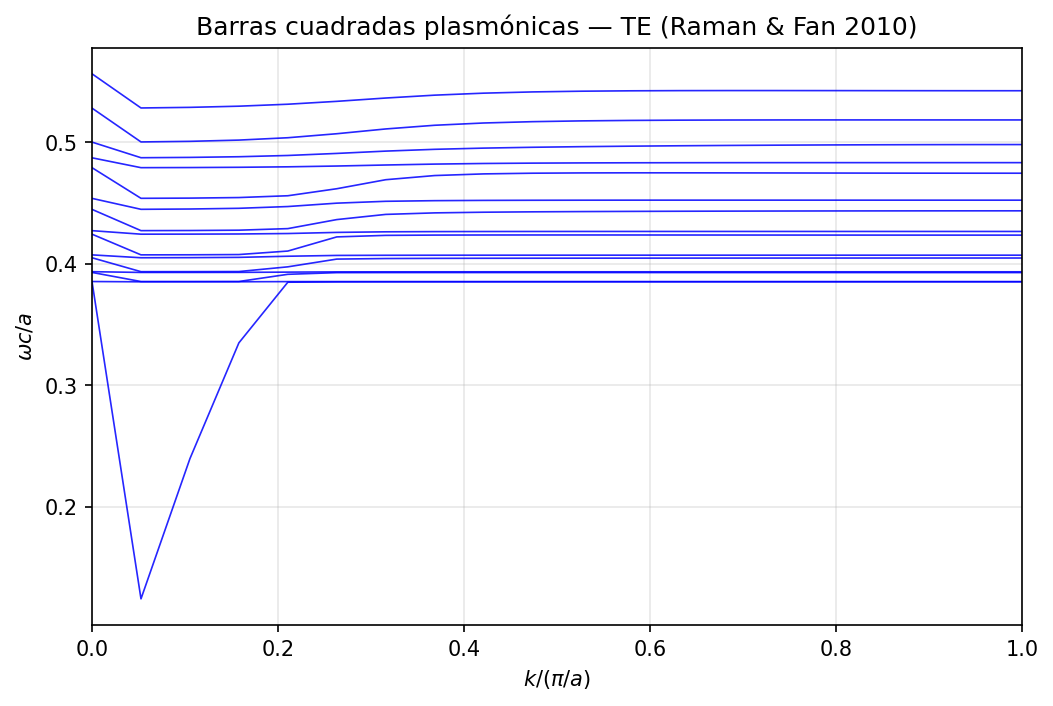
\includegraphics[width=0.85\textwidth]{../figures/square_rods_TE_bands.png}%
  }{%
    \fbox{\parbox{0.8\textwidth}{\centering Ejecutar \texttt{examples/square\_rods\_TE.py}}}%
  }
  \caption{Estructura de bandas TE para barras cuadradas plasmónicas.}
\end{figure}

\begin{figure}[htbp]
  \centering
  \IfFileExists{../figures/lossy_case_comparison.png}{%
    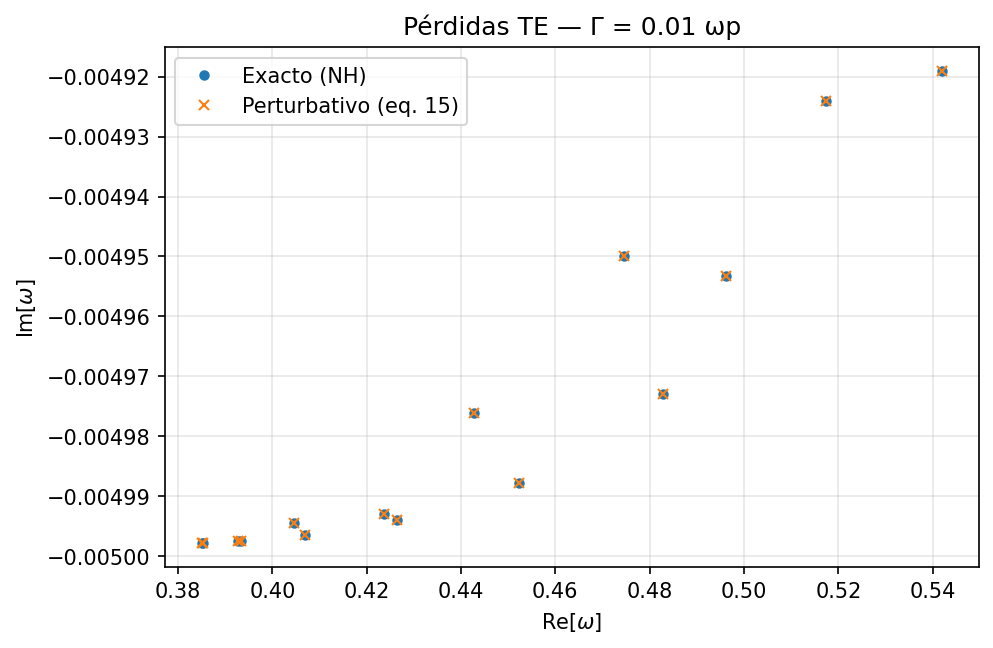
\includegraphics[width=0.85\textwidth]{../figures/lossy_case_comparison.png}%
  }{%
    \fbox{\parbox{0.8\textwidth}{\centering Ejecutar \texttt{examples/lossy\_case.py}}}%
  }
  \caption{Comparación de pérdidas modales: exacto vs perturbativo.}
\end{figure}

\section{Conclusiones}

La implementación Python reproduce la formulación del paper con código
modular, validaciones automatizadas y ejemplos reproducibles. Extiende el
proyecto C++ previo con mayor flexibilidad para investigación académica.

\bibliographystyle{plain}
\bibliography{bibliography}

\end{document}
